\chapter{Border Gateway Protocol (BGP)}
\section{Exterior Routing with BGP}
\begin{itemize} 
\item The Border Gateway Protocol (BGP) is the protocol backing the core routing decisions.
\item On the Internet. It maintains a table of IP networks or prefixes which designate network reachability among autonomous systems (AS). It is described as a path vector protocol.
\item BGP does not use traditional Interior Gateway Protocol (IGP) metrics, but makes routing decisions based on path, network policies and/or rule sets
\section{ Build the topology with Kathara.}
\end{itemize}
\begin{figure}[H]
\centering
  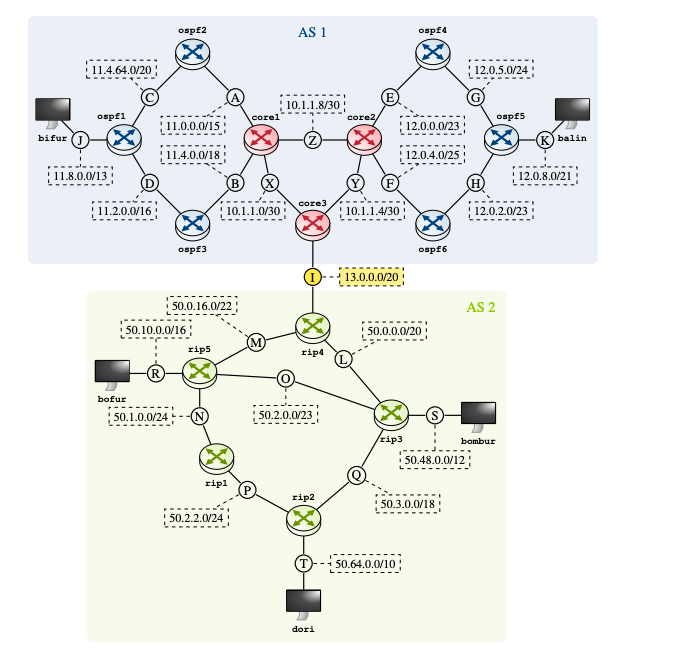
\includegraphics[width=0.9\textwidth]{Images/BGP_Topology.png}
  \caption{BGP Topology}
  \label{fig }
\end{figure}
\section{Building the topology for BGP network}
\subsection{Step 1. Remove kili at the edge of each network and connect core3 with rip4 over CD I}
\begin{itemize}
\item Combine the two lab.conf files of previous networks into a single lab file and remove killi in the lab.conf file.
\end{itemize}
\subsection{ Choose IP address of the network 13.0.0.0/20 and add CD I to rip4}
\begin{itemize}
\item IP address in rip4.startup file which connects to core3 over collision domain 13.0.0.0/20
\item  ip addr add 13.0.0.4/20 brd + dev eth0
\begin{figure}[H]
\centering
  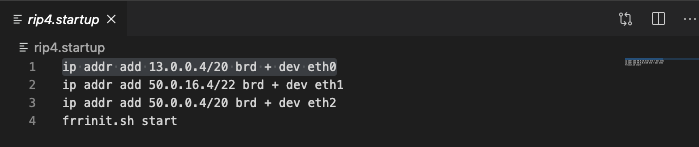
\includegraphics[width=0.9\textwidth]{Images/rip4.startup.png}
  \caption{rip4.startup file}
  \label{fig }
\end{figure}
\item IP address in core3.startup file which connects to core3 over collision domain 13.0.0.0/20
\item ip addr add 13.0.0.3/20 brd + dev eth2
\end{itemize}
\begin{figure}[H]
\centering
  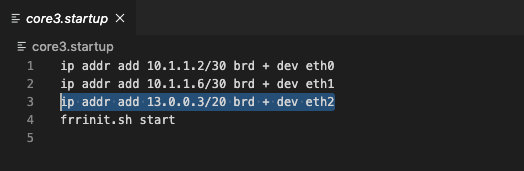
\includegraphics[width=0.9\textwidth]{Images/core3.startup.png}
  \caption{Core3.startup file}
  \label{fig }
\end{figure}
\section{Configure the BGP peering between both Areas, where AS 1 is responsible for the OSPF network and AS 2 for RIP}
\section{BGP configuration in core3}
\begin{itemize}
    \item We must create bgpd.conf file in core3
    \begin{figure}[H]
\centering
  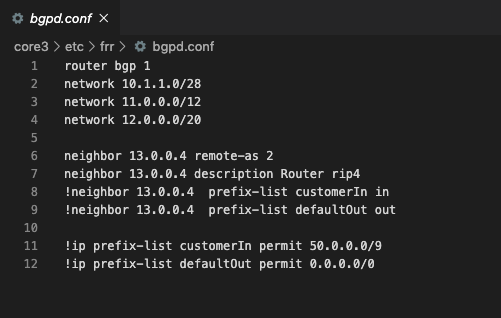
\includegraphics[width=0.9\textwidth]{Images/BGPD_core3.conf.png}
  \caption{BGPD.conf file of Core3}
  \label{fig }
\end{figure}
\subsection{ router bgp 1 : this specifies that the core3 is in area one . That is OSPF network is completely considered area 1}
\end{itemize}
\subsection{IP Addresses of OSPF network which includes IP address of all 3 areas(networks) of the OSPF network}
\begin{itemize}
\item network 10.1.1.0/28 : Backbone area 3.3.3.3(core 1 core2 core3)
\item network 11.0.0.0/12 : Area 1.1.1.1 (bgp1 bgp2 bgp3)
\item network 12.0.0.0/20 : Area 2.2.2.2 (bgp4 bgp5 bgp6)
\end{itemize}
\subsection{Neighbour of core3}
\begin{itemize}
\item neighbor 13.0.0.4 remote-as 2 : Specifies the ip of rip4 and considers its area as 2
\item neighbor 13.0.0.4 description Router rip4 : Specifies the name of the neighbour that is rip4
\end{itemize}
\section{BGP configuration in rip4}
\begin{itemize}
    \item We must create bgpd.conf file in rip4
    \begin{figure}[H]
\centering
  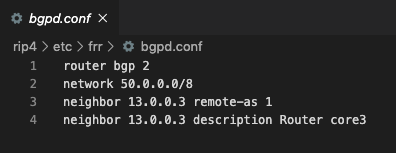
\includegraphics[width=0.9\textwidth]{Images/BGPD_rip4.conf.png}
  \caption{BGPD.conf file of rip4}
  \label{fig }
\end{figure}
\subsection{ router bgp 2 : this specifies that the rip4 is in area 2. That is RIP network is completely considered as area 2}
\end{itemize}
\subsection{IP Addresses of RIP network which includes IP address of all  areas(networks) of the RIP network}
\begin{itemize}
\item network 50.0.0.0/8 : Includes all the RIP network routers and host
\end{itemize}
\subsection{Neighbour of rip4}
\begin{itemize}
\item neighbor 13.0.0.3 remote-as 1 : Specifies the ip of core3 and considers its area as 1
\item neighbor 13.0.0.3 description Router core3 : Specifies the name of the neighbour that is core3
\end{itemize}
\section{Adjust the announcements, so that all hosts of both Areas can reach each other}
\subsection{Declare BGPD in both daemon file}
\begin{figure}[H]
\centering
  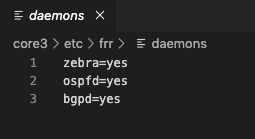
\includegraphics[width=0.9\textwidth]{Images/Deamon.png}
  \caption{Deamon file }
  \label{fig }
\end{figure}
\section{Adding static routes wherever needed to ensure global connectivity.}
\begin{itemize}
    \item In OSPFD file of Core3 remove interfaces and areas as it is already declared in bgpd file
    \item Declare redistribute bgp
\end{itemize}
\begin{figure}[H]
\centering
  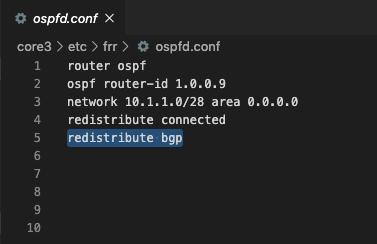
\includegraphics[width=0.9\textwidth]{Images/ospfd.png}
  \caption{Deamon file }
  \label{fig }
\end{figure}
\begin{itemize}
    \item In RIPD file of rip4 mention the network 50.0.0.0/20 and
network 50.0.16.0/22
    \item Declare redistribute bgp
\end{itemize}
\begin{figure}[H]
\centering
  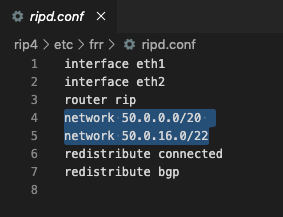
\includegraphics[width=0.9\textwidth]{Images/ripd.png}
  \caption{RIPD file }
  \label{fig }
\end{figure}
\section{Checking connectivity among all hosts of both Areas}
\begin{itemize}
    \item Checking connectivity between Bifur and Bombur (Bifur belongs to OSPFD and Bombur belongs to RIPD networks)
\end{itemize}
\begin{figure}[H]
\centering
  \includegraphics[width=0.9\textwidth]{Images/.png}
  \caption{Connectivity between Bifur and Bombur  }
  \label{fig }
\end{figure}
\begin{itemize}
    \item Checking connectivity between Balin and Dori
\end{itemize}
\begin{figure}[H]
\centering
  \includegraphics[width=0.9\textwidth]{Images/.png}
  \caption{Connectivity between Balin and Dori  }
  \label{fig }
\end{figure}
\begin{itemize}
    \item Checking connectivity between Balin and Bombur
\end{itemize}
\begin{figure}[H]
\centering
  \includegraphics[width=0.9\textwidth]{Images/.png}
  \caption{Connectivity between Balin and Bombur  }
  \label{fig }
\end{figure}








\section{Inspecting the routing tables of rip4 and core3 and explain, how the peering is done with BGP}
\subsection{Routing Table of Rip4}
\begin{figure}[H]
\centering
  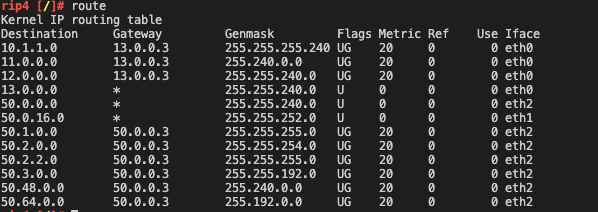
\includegraphics[width=1.4\textwidth]{Images/route rip4.png}
  \caption{Routing Table of Rip4  }
  \label{fig }
\end{figure}
\begin{itemize}
    \item In Rip4 routing table the OSPFD network in connected from core3 which is the bgpd router 
    \item RIP4 is connecting to 10.1.1.0 ip address which covers all the ip address of the backbone area (core1,core2,core3) of OSPfD network through the gateway 13.0.0.3 which is the ip address of Core3 
\end{itemize}
\begin{figure}[H]
\centering
  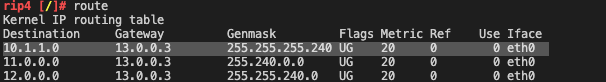
\includegraphics[width=1.3\textwidth]{Images/rip4 routing to core3.png}
  \caption{Connecting from rip4 to core3 network}
  \label{fig }
\end{figure}
\begin{itemize}
    \item Similarly RIP4 is connecting to 11.0.0.0 and 12.0.0.0 ip address which covers all the ip address of Bifur, Ospf1, Ospf2 ,Ospf3 ,core1 and Core2, Ospf4, Ospf5, Ospf6, Balin of OSPFD network through the gateway 13.0.0.3 which is the ip address of Core3 
\end{itemize}
\begin{itemize}
    \item In Rip4 routing table the RIP network in connected from rip4 which is the bgpd router via rip3 as gateway.
    \item RIP4 is connecting to all the collision domain ip address which covers all the ip address of RiP network via rip3(50.0.0.3 ).
    \end{itemize}
 \begin{figure}[H]
\centering
  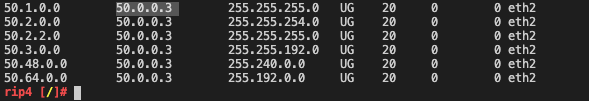
\includegraphics[width=1.3\textwidth]{Images/rip4 to ripd.png}
  \caption{Connecting from rip4 to RIPD network}
  \label{fig }
\end{figure}  
\subsection{Routing Table of Core3}
 \begin{figure}[H]
\centering
  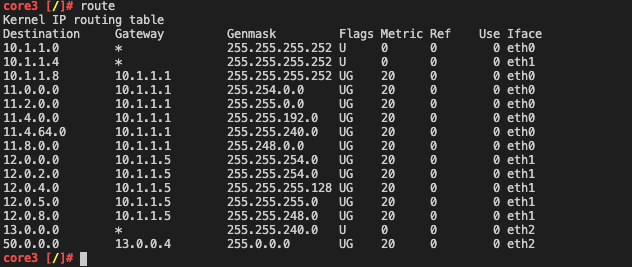
\includegraphics[width=1.3\textwidth]{Images/Routing table of core3.png}
  \caption{Routing Table of Core3}
  \label{fig }
\end{figure}
\begin{itemize}
    \item In Core3 routing table the RIP network is connected to Bgpd network(50.0.0.0) from rip4 which is the Bgpd router via rip4(13.0.0.4) as gateway.
    \end{itemize}
 \begin{figure}[H]
\centering
  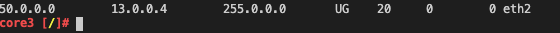
\includegraphics[width=1.3\textwidth]{Images/core3 route 2.png}
  \caption{Connecting between OSPFD network and RIPD network}
  \label{fig }
\end{figure}
\begin{itemize}
    \item In Core3 routing table the all the OSFD routers and host are connected as the collision domain ip address is taken of the entire network via 10.1.1.1 (core1) and 10.1.1.5(core5) as gateway respectively.
    \item Core1 Ospfd1 ospfd2 ospfd3 and Bifur are connected via 10.1.1.1 as gatway.
    \item Core2 Ospfd4,Ospfd5,Ospfd6,Balin are connected via 10.1.1.5 as gateway.
    \end{itemize}
 \begin{figure}[H]
 \centering
  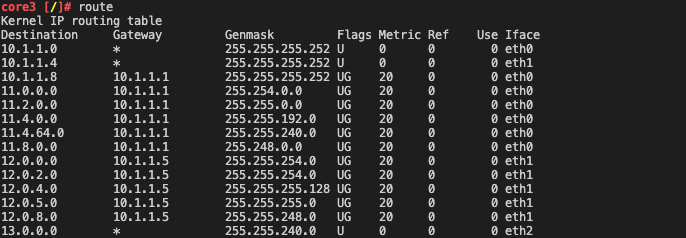
\includegraphics[width=1.3\textwidth]{Images/core3 route3.png}
  \caption{Connecting Core3 to OSPFD network}
  \label{fig }
\end{figure}
\begin{itemize}
    \item And this is how the bgpd routers helps to connect the two networks and hence we can ping from any host of Ospfd network to host of RIPD network
\end{itemize}